\section{Color-Adaptive Decomposition}
\label{sec:volumetric:acd}

In this section, we present methods for more efficient decomposition from color-volume to binary-volume, efficiency here refering to the number of binary depth planes that are used to represent a color depth plane. 

\subsection{Motivation}
In the method presented in Sec. \todo{find the section number}, each color voxel was decomposed into the nearest 24 binary depth planes. Since our display's LEDs can change color and intensity over a very large range on a per-binary frame basis, we don't need to limit our display to a fixed pattern of LED colors and intensities or to 8 bits-per-color. A more optimum decomposition method might use fewer number of binary voxels to represent the same color voxel. It is useful to reduce the number of binary voxels that represent each color voxel for the following reasons:

\begin{enumerate}
    \item This will reduce the depth-blur associated with each color voxel.
    \item This may be useful for more compact prototypes because the more compact DMD projectors have a slower refresh rate than the DMD projector used in our display.
    \item We may be able to achieve High Dynamic Range imagery.
    \item With fewer number of binary voxels representing each color voxel, we can represent objects that are transparent and closer to each other than with the fixed pipeline decomposition. With the fixed pipeline decomposition, we can not represent objects along the same depth that are closer than $3 \times \text{color bit-depth}$.
\end{enumerate}

\subsection{Approach}
The basic idea behind the color adaptive decomposition methods explored here is that of error propagation or diffusion. 
Starting at the nearest depth plane, we consider the slice of the color volume and do the best of representing it with a binary image and an arbitrary LED color. 
Unavoidably, there will be errors, which are propagated onto the next depth plane. 
At the next depth plane, the current depth's slice of the color volume and the propagated errors are added and considered as the target image for the decomposition.
The pseudo-code for this approach is given in Algorithm.~\ref{alg:colorAdaptiveMethodOne}.

Let $R$ denote residue, $T$ denote the target image, $A$ denote the actual reconstruction, $L$ denote the LEDs, $B$ denote the binary image, and $V$ denote the volume. Then, 

\begin{algorithm}
    \caption{Outline of error propagation appoach}
    \label{alg:colorAdaptiveMethodOne}
    \hspace*{\algorithmicindent}\textbf{Input:} $V$\\
    \hspace*{\algorithmicindent}\textbf{Output:} $B, L$
    \begin{algorithmic}[1]
        \STATE{$R \gets \text{zeros}$}
        \FOR{$d \gets 1$ \TO $\numPlanes$}
        \STATE{$I \gets V \lbrack :,:,d \rbrack $}
        \STATE{$T \gets I + R$}
        \STATE{${(B_d,L_d)} \gets \text{Decompose$(T)$}$}
        \STATE{$R \gets T - \text{Reconstruct$(B_d, L_d)$}$}
        \ENDFOR
    \end{algorithmic}
\end{algorithm}

The methods explored here differ from each other in the way the target image at each depth is decomposed, i.e., the \emph{Decompose} function in Algorithm.~\ref{alg:colorAdaptiveMethodOne}.
In the sections below, we explore some possible ways to decompose the target image at each depth.
For each of the methods below, the decomposition step tries to minimize the L2-norm between the decomposition and the target images:
\begin{equation}
    \argmin_{B_d,L_d} ||T - \text{Reconstruct}(B_d, L_d) ||^2
\end{equation}

However, the problem with trying to decompose a 24-bit target RGB image into a 1-bit DMD image and an RGB LED value is that:
\begin{enumerate}
    \item Because the DMD pattern is common for the three color channels, the decomposition is not separable among the color-channels, e.g., a particular DMD pattern may have very low loss for the red channel but very high for the green channel such that the combined error might be lesser than completely leaving out green channel. 
    \item Something to do with binarization. The threshold determines whether you under-expose or over-expose. When you under-expose, the errors are propagated much farther away from the slice which caused the error.
    \item 
\end{enumerate}

\subsubsection{Brute-force}
In this method, we calculate the decomposition for every combination of color channel. 
These are the difference combinations of color channels: $O_1 = $\{ 1, 0, 0 \}, $O_2 = $ \{ 0, 1, 0 \}, $O_3 = $ \{ 0, 0, 1 \}, $O_4 = $ \{ 1, 1, 0 \}, $O_5 = $ \{ 1, 0, 1 \}, $O_6 = $ \{ 0, 1, 1 \}, $O_7 = $ \{ 1, 1, 1 \}, where 0 indicates that the color channel is not considered for the optimization and 1 indicatest that the color channel is considered for the optimization. 

See Algorithm~\ref{alg:bruteforce} for a pseudo-code for this approach. A step-wise explanation for the algorithm follows:
\begin{itemize}
    \item Lines 1-2: At each depth plane, we assign the target image by adding the previous residual to the current depth plane's image. We split this target image ($T$) into its color channels $(C_1, C_2, C_3))$ because we process the color channel's independently in the initial part of the algorithm to estimate the common optimal binary image.
    \item Line 3: In the outer for-loop, we consider each of the seven possible options for whether an LED is on or off, i.e., $O_1$, $O_2$, ..., $O_7$, and save these calculated values: LED values ($L_i$), binary pattern ($B_i$), the reconstructed image ($S_i$), the residual ($R_i$), and the energy or loss ($E_i$).
    \item Lines 5-13: calculate the best LED value and binary pattern when each color channel is considered independently and in accordance with whether that color channel's LED should be on or off. If that color channel's LED should be off, then the LED value for that color channel is set to 0 and the binary pattern is set to all ones. If however the LED should be on, the LED value is calculated as the mean value of the non-zero pixel values of that color channel and the binary pattern is calculated by thresholding the pixel values divided by the calculated LED value. Ideally, this threshold should be set to 1. \todo{What is the threshold value used?}.
    \item Line 14: Since the DMD pattern is common to all three color channels, we need to calculate the common binay pattern by simply multiplying together all the color channel's binay patterns. 
    \item Lines 15-24: Because the common binary pattern may be different from each of the color channel's binary patterns, we need to calculate the new optimum LED values. This for-loop accomplishes that by assigning each LED value to the minimum pixel value in its color channel.
    \item Lines 27-30: We find which option resulted in the least energy and output that option's binary pattern, LED values, and residual image. 
\end{itemize}

\begin{algorithm}
    \caption{Brute-force color decomposition}
    \label{alg:bruteforce}
    \hspace*{\algorithmicindent}\textbf{Input:} $T, R$\\
    \hspace*{\algorithmicindent}\textbf{Output:} $B, L, R$
    \begin{algorithmic}[1]
        \STATE{$T \gets I + R$}
        \STATE{$ \{C_1, C_2, C_3 \} \gets \text{split}(T)$}
        \FOR{$i \gets 1$ \TO $7$}
        \FOR{$j \gets 1$ \TO $3$}
        \IF{$O_i[j] == 0$}
        \STATE{$L_j \gets 0$}
        \STATE{$B_j \gets I_{\text{ones}}$}
        \ELSE
        \STATE{$L_j \gets \mu\left( \{ C_j : C_j \neq 0 \} \right)$}
        \STATE{$B_j \gets \text{sgn}\left( \frac{C_j}{L_j} - T \right)$}
        \ENDIF
        \ENDFOR
        \STATE{$B_i \gets B_1 \cdot B_2 \cdot B_3$}
        \FOR{$j \gets 1$ \TO $3$}
        \IF{$O_i[j] == 0$}
        \STATE{$L_j \gets 0$}
        \ELSE
        \STATE{$C_j' \gets C_j \cdot B_i$}
        \STATE{$L_j \gets \min \left( \{ C_j' : C_j' \neq 0 \} \right)$}
        \ENDIF
        \ENDFOR
        \STATE{$L_i \gets \{L_r, L_g, L_b \}$}
        \STATE{$S_i \gets \text{Reconstruct}(B_i,L_i)$}
        \STATE{$R_i \gets T - S_i$}
        \STATE{$E_i \gets \text{Loss}(R_i)$}
        \ENDFOR
        \STATE{$k \gets \argmin(E_1,E_2,\ldots,E_7)$}
        \STATE{$B \gets B_k$}
        \STATE{$L \gets L_k$}
        \STATE{$R \gets R_k$}
    \end{algorithmic}
\end{algorithm}

\subsubsection{Highest Energy Channel Minimization}
\begin{algorithm}
    \caption{Highest Energy Channel Minimization}
    \label{alg:highest_energy_channel_minimization}
    \hspace*{\algorithmicindent}\textbf{Input:} $T, R$\\
    \hspace*{\algorithmicindent}\textbf{Output:} $B, L, R$
    \begin{algorithmic}[1]
        \STATE{$T \gets I + R$}
        \STATE{$ \{C_1, C_2, C_3 \} \gets \text{split}(T)$}
        \STATE{$\{ E_1, E_2, E_3 \} \gets Loss(\{ C_1, C_2, C_3 \})$}
        \STATE{$k \gets i:E_i = \max(E_1, E_2, E_3)$}
        \STATE{$L \gets \{0, 0, 0 \}$}
        \STATE{$ L_k \gets \mu(C_k:C_k \neq 0) $}
        \STATE{$B \gets \text{sgn}(\frac{C_k}{L_k} - T)$}
        \STATE{$S \gets \text{Reconstruct}(B,L)$}
        \STATE{$R \gets T - S$}
    \end{algorithmic}
\end{algorithm}

See Algorithm~\ref{alg:highest_energy_channel_minimization} for a pseudo-code for this approach. A step-wise explanation for the algorithm follows:
\begin{itemize}
    \item Line 1: At each depth plane, we assign the target image by adding the previous residual to the current depth plane's image. 
    \item Line 2: Split the target image ($T$) into its color channels $(C_1, C_2, C_3))$ because we process the color channel's independently.
    \item Line 3: Calculate the energy of each color channel.
    \item Line 4: Find the color channel that has the maximum energy. For the rest of the algorithm, it is only this color channel that is of interest to us. The other two color channels are ignored.
    \item Lines 5-6: Each LED color is first assigned to 0. Then, only for the color channel of maximum energy, the LED color is calculated as the mean of the non-zero pixel values of that color channel.
    \item Line 7: The binary image is calculated by thresholding the color channel of maximum energy channel against the calculated LED color.
    \item Line 8-9: Calculating the reconstructed image and the residual image.
 \end{itemize}


\subsubsection{Projected Gradient}
\label{sec:acd_projected_gradient}
This approach is based on non-negative matrix factorization methods as used in recent compressive displays~cite{Wetzstein2012,Huang2015Light,huang2017mixed}. 
However, the previous papers were concerned with decomposing a continuous-valued image into two or more continuous-valued images. 
Here, by continuous, we mean that the values are considered to be in continuous domain even through in a computer they may be represented by an 8-bit per color channel image. 
However, in our display, we need to decompose continuous-valued images (slices of the color volume) into a binary image and a continuous-valued triplet for the RGB LED. 
This is a significantly harder problem because it is a combination of the traditional optimization as explored by non-negative matrix factorizatin algorithms and combinatorial optimization which has not been explored previously in context of computational displays. 
In this section, we derive the update rules for non-negative matrix factorization algorithms, and we write down the algorithm and explain it.
We shall see later in the \todo{results section} that this algorithm does poorly in terms of visual quality.

\paragraph{Newton's method adapted for optimization}
Non-negative matrix factorization's update rules can be understood from studying Newton's method adapted for optimization:

Taylor expansion:
\begin{equation}
  f(x) = f(x_0) + \Delta f'(x_0) + \frac{\Delta x^2 f''(x_0)}{2} + ...
\end{equation}
where $\Delta x = x - x_0$.

Let us consider only first three terms of the Taylor expansion. We differentiate the above equation wrt $\Delta x$ to determine the optimum step size to guarantee fast convergence.

\begin{equation}
  \frac{d f(x)}{d(\Delta x)} = \frac{d \left( f(x_0) + \Delta f'(x_0) + \frac{\Delta x^2 f''(x_0)}{2}\right)}{d(\Delta x)} 
\end{equation}

\begin{equation}
  0 = f'(x_0) + \Delta x f''(x_0)
\end{equation}

Rearranging:
\begin{equation}
  \Delta x = - \frac{f'(x_0)}{f''(x_0)}
\end{equation}

Then,
\begin{equation}
  x_{n+1} = x_n - \frac{f'(x_0)}{f''(x_o)}
\end{equation}

\paragraph{Applying Newton's method for our problem}

This is the mathematics for the matlab file named \emph{adaptive\_color\_decomposition\_all\_channels.m}.

Now, let us apply Newton's method to our problem. Let us first denote the color volume by $V_c$, the
binary volume by $V_b$, the color sub-volume image to be $C$, the binary subvolume image to be
$B$, the LED color and brightness associated with $B$ to be $\alpha$. We now define the energy
function that is to be optimized:

\begin{equation}
  E = ||C - \alpha B||^2 = ||C^T - \alpha B^T||^2
\end{equation}

Note that the energy function is the L2-norm of the residual, $R$, defined as:
\begin{equation}
  R = C - \alpha B = C^T - \alpha B^T
\end{equation}

Deriving update rule for $B$
Expanding $E = ||C^T - \alpha B^T||^2$:
\begin{equation}
  E = C^TC - 2C^T\alpha B + \alpha^2 B^T B
\end{equation}

\begin{equation}
  \frac{dE}{dB} = -2\alpha C^T + 2\alpha^2 B^T
\end{equation}

and
\begin{equation}
  \frac{d^2E}{dB^2} = 2\alpha
\end{equation}

Then,
\begin{equation}
  \Delta B = \frac{2\alpha C^T - 2 \alpha^2 B^T}{2 \alpha^2} = \frac{C^T - \alpha B^T}{\alpha} = \frac{R^T}{\alpha}
\end{equation}

and
\begin{equation}
  B_{n+1} = B_n + \frac{R^T}{\alpha}
  \label{eq:binary_image_update}
\end{equation}

Deriving update rule for $\alpha$:
Expanding $E = ||C^T - \alpha B^T||^2$:
\begin{equation}
  E = C^TC - 2C^T\alpha B + \alpha^2 B^T B
\end{equation}

\begin{equation}
  \frac{dE}{d \alpha} = - 2 C^TB + 2 \alpha B^TB
\end{equation}

\begin{equation}
  \frac{d^2E}{d \alpha^2} = 2B^TB
\end{equation}

Then, 
\begin{equation}
  \Delta \alpha = \frac{2 C^TB - 2\alpha B^TB}{2 B^TB} = \frac{C^TB - \alpha B^TB}{B^TB} = \frac{R^TB}{B^TB}
\end{equation}

and
\begin{equation}
  \alpha_{n+1} = \alpha_n + \frac{R^TB}{B^TB}
  \label{eq:led_update}
\end{equation}

\begin{algorithm}
    \caption{Projected Gradients}
    \label{alg:projected_gradients}
    \hspace*{\algorithmicindent}\textbf{Input:} $T, R$\\
    \hspace*{\algorithmicindent}\textbf{Output:} $B, L, R$
    \begin{algorithmic}[1]
        \STATE{$T \gets I + R$}
        \STATE{$ \{C_1, C_2, C_3 \} \gets \text{split}(T)$}
        \FOR{$j \gets 1$ \TO $3$}
        \STATE{$L_j \gets \mu(C_j:C_j \neq 0)$}
        \STATE{$D_j \gets \frac{C_j}{L_j}$}
        \ENDFOR
        \STATE{$B \gets \text{sgn}(D_1 + D_2 + D_3 - T)$}
        \STATE{$S \gets \text{Reconstruct}(B,L)$}
        \STATE{$R \gets T - S$}
        \FOR{$j \gets 1$ \TO $2$}
        \FOR{$j \gets 1$ \TO $3$}
        \STATE{$L_j \gets L_j + \frac{R_j \cdot B}{B \cdot B}$}
        \ENDFOR
        \STATE{$S \gets \text{Reconstruct}(B,L)$}
        \STATE{$R \gets T - S$}
        \FOR{$j \gets 1$ \TO $3$}
        \STATE{$D_j \gets \frac{R_j}{L_j}$}
        \ENDFOR
        \STATE{$B \gets \text{sgn}(B + D_1 + D_2 + D_3)$}
        \STATE{$S \gets \text{Reconstruct}(B,L)$}
        \STATE{$R \gets T - S$}
        \ENDFOR
    \end{algorithmic}
\end{algorithm}

See Algorithm~\ref{alg:projected_gradients} for a pseudo-code for this approach. A step-wise explanation for the algorithm follows:
\begin{itemize}
    \item Line 1: At each depth plane, we assign the target image by adding the previous residual to the current depth plane's image. 
    \item Line 2: Split the target image ($T$) into its color channels $(C_1, C_2, C_3))$ because we process the color channel's independently.
    \item Lines 3-6: For each color channel, initialize the LED value to be the mean of that color channel's non-zero pixel values. Assuming that the DMD image is a per-channel continuous-valued image, calculate the initial guess by normalizing the color image by the mean of the color image.  
    \item Line 7: Combine the per-channel continuous-valued images into a binary image by adding and thresholding. 
    \item Line 8-9: Calculate the reconstructed image and the residual image.
    \item Line 10,22: for-loop for two iterations of the non-negative matrix factorization algorithm.
    \item Lines 11-13: Update the LED values according to Eq.~\ref{eq:led_update}.
    \item Lines 14-15: Calculate the reconstructed image and the residual image.
    \item Lines 16-18: Assuming that the DMD image is a per-channel continuous-valued image, calculate the gradient according to Eq.~\ref{eq:binary_image_update}.
    \item Line 19: Combine the per-channel continuous-valued image-gradients into a binary image by adding and thresholding.
    \item Lines 20-21: Calculate the reconstructed image and the residual image.
\end{itemize}

\subsubsection{Heuristic}
\label{sec:acd_heuristis}
This approach is a judicious combination of the brute-force approach (which yields the best image quality, least number of binary voxels, but longest runtime) and the projected gradients approach (which yields very poor image quality, comparable number of binary voxels, but fast runtimes). 
In this approach, we treat treat the problem as a combination of a combinatorial optimization (for selecting which combination of color channels the DMD image and LEDs should try to address) and continous-valued optimization (for selecting the LED values). 
In this approach, the combinatorial optimization portion (selecting the combination of color channels to address) automatically determines the DMD pattern too.
See Algorithm~\ref{alg:heuristics} for a pseudo-code for this approach. A step-wise explanation for the algorithm follows:
\begin{itemize}
    \item Line 1: At each depth plane, we assign the target image by adding the previous residual to the current depth plane's image. 
    \item Line 2: Split the target image ($T$) into its color channels $(C_1, C_2, C_3))$ because we process the color channel's independently.
    \item Lines 3-6: For each color channel, initialize the LED value to be the mean of that color channel's non-zero pixel values. Assuming that the DMD image is a per-channel continuous-valued image, calculate the initial guess by normalizing the color image by the mean of the color image.  
    \item Line 7: Combine the per-channel continuous-valued images into a binary image by adding and thresholding. 
    \item Line 8-9: Calculate the reconstructed image and the residual image.
    \item Line 10,22: for-loop for two iterations of the non-negative matrix factorization algorithm.
    \item Lines 11-13: Update the LED values according to Eq.~\ref{eq:led_update}.
    \item Lines 14-15: Calculate the reconstructed image and the residual image.
    \item Lines 16-18: Assuming that the DMD image is a per-channel continuous-valued image, calculate the gradient according to Eq.~\ref{eq:binary_image_update}.
    \item Line 19: Combine the per-channel continuous-valued image-gradients into a binary image by adding and thresholding.
    \item Lines 20-21: Calculate the reconstructed image and the residual image.
\end{itemize}

\begin{algorithm}
    \caption{Heuristic approach}
    \label{alg:heuristics}
    \hspace*{\algorithmicindent}\textbf{Input:} $T, R$\\
    \hspace*{\algorithmicindent}\textbf{Output:} $B, L, R$
    \begin{algorithmic}[1]
        \STATE{$T \gets I + R$}
        \STATE{$ \{C_1, C_2, C_3 \} \gets \text{split}(T)$}
        \FOR{$j \gets 1$ \TO $3$}
        \STATE{$L_j \gets \mu(C_j:C_j \neq 0)$}
        \STATE{$B_j \gets \text{sgn}(\frac{C_j}{L_j} - T)$}
        \ENDFOR
        \FOR{$i \gets 1$ \TO $7$}
        \STATE{$D_i \gets I_\text{ones}$}
        \FOR{$j \gets 1$ \TO $3$}
        \IF{$O_i[j] == 1$}
        \STATE{$D_i \gets D_i \cdot B_j$}
        \ENDIF
        \ENDFOR
        \STATE{$E_i \gets \text{reduce\_sum}(D_i)$}
        \ENDFOR
        \STATE{$k \gets \argmin(E_1,E_2,\ldots,E_7)$}
        \STATE{$B \gets D_k$}
        \STATE{$L \gets L \cdot O_k$}
        \STATE{$S \gets \text{Reconstruct}(B,L)$}
        \STATE{$R \gets T \cdot O_k - S$}
        \FOR{$j \gets 1$ \TO $3$}
        \STATE{$L_j \gets L_j + \frac{R_j \cdot B}{B \cdot B}$}
        \ENDFOR
        \STATE{$S \gets \text{Reconstruct}(B,L)$}
        \STATE{$R \gets T - S$}
    \end{algorithmic}
\end{algorithm}

\subsection{Results}
\begin{enumerate}
  \item PSNR of reconstruction
  \item SSIM of reconstruction
  \item Number of binary voxels
  \item Transparencies
  \item PSNR of focal stacks
  \item SSIM of focal stacks
\end{enumerate}

\begin{figure}[h!]
\centering
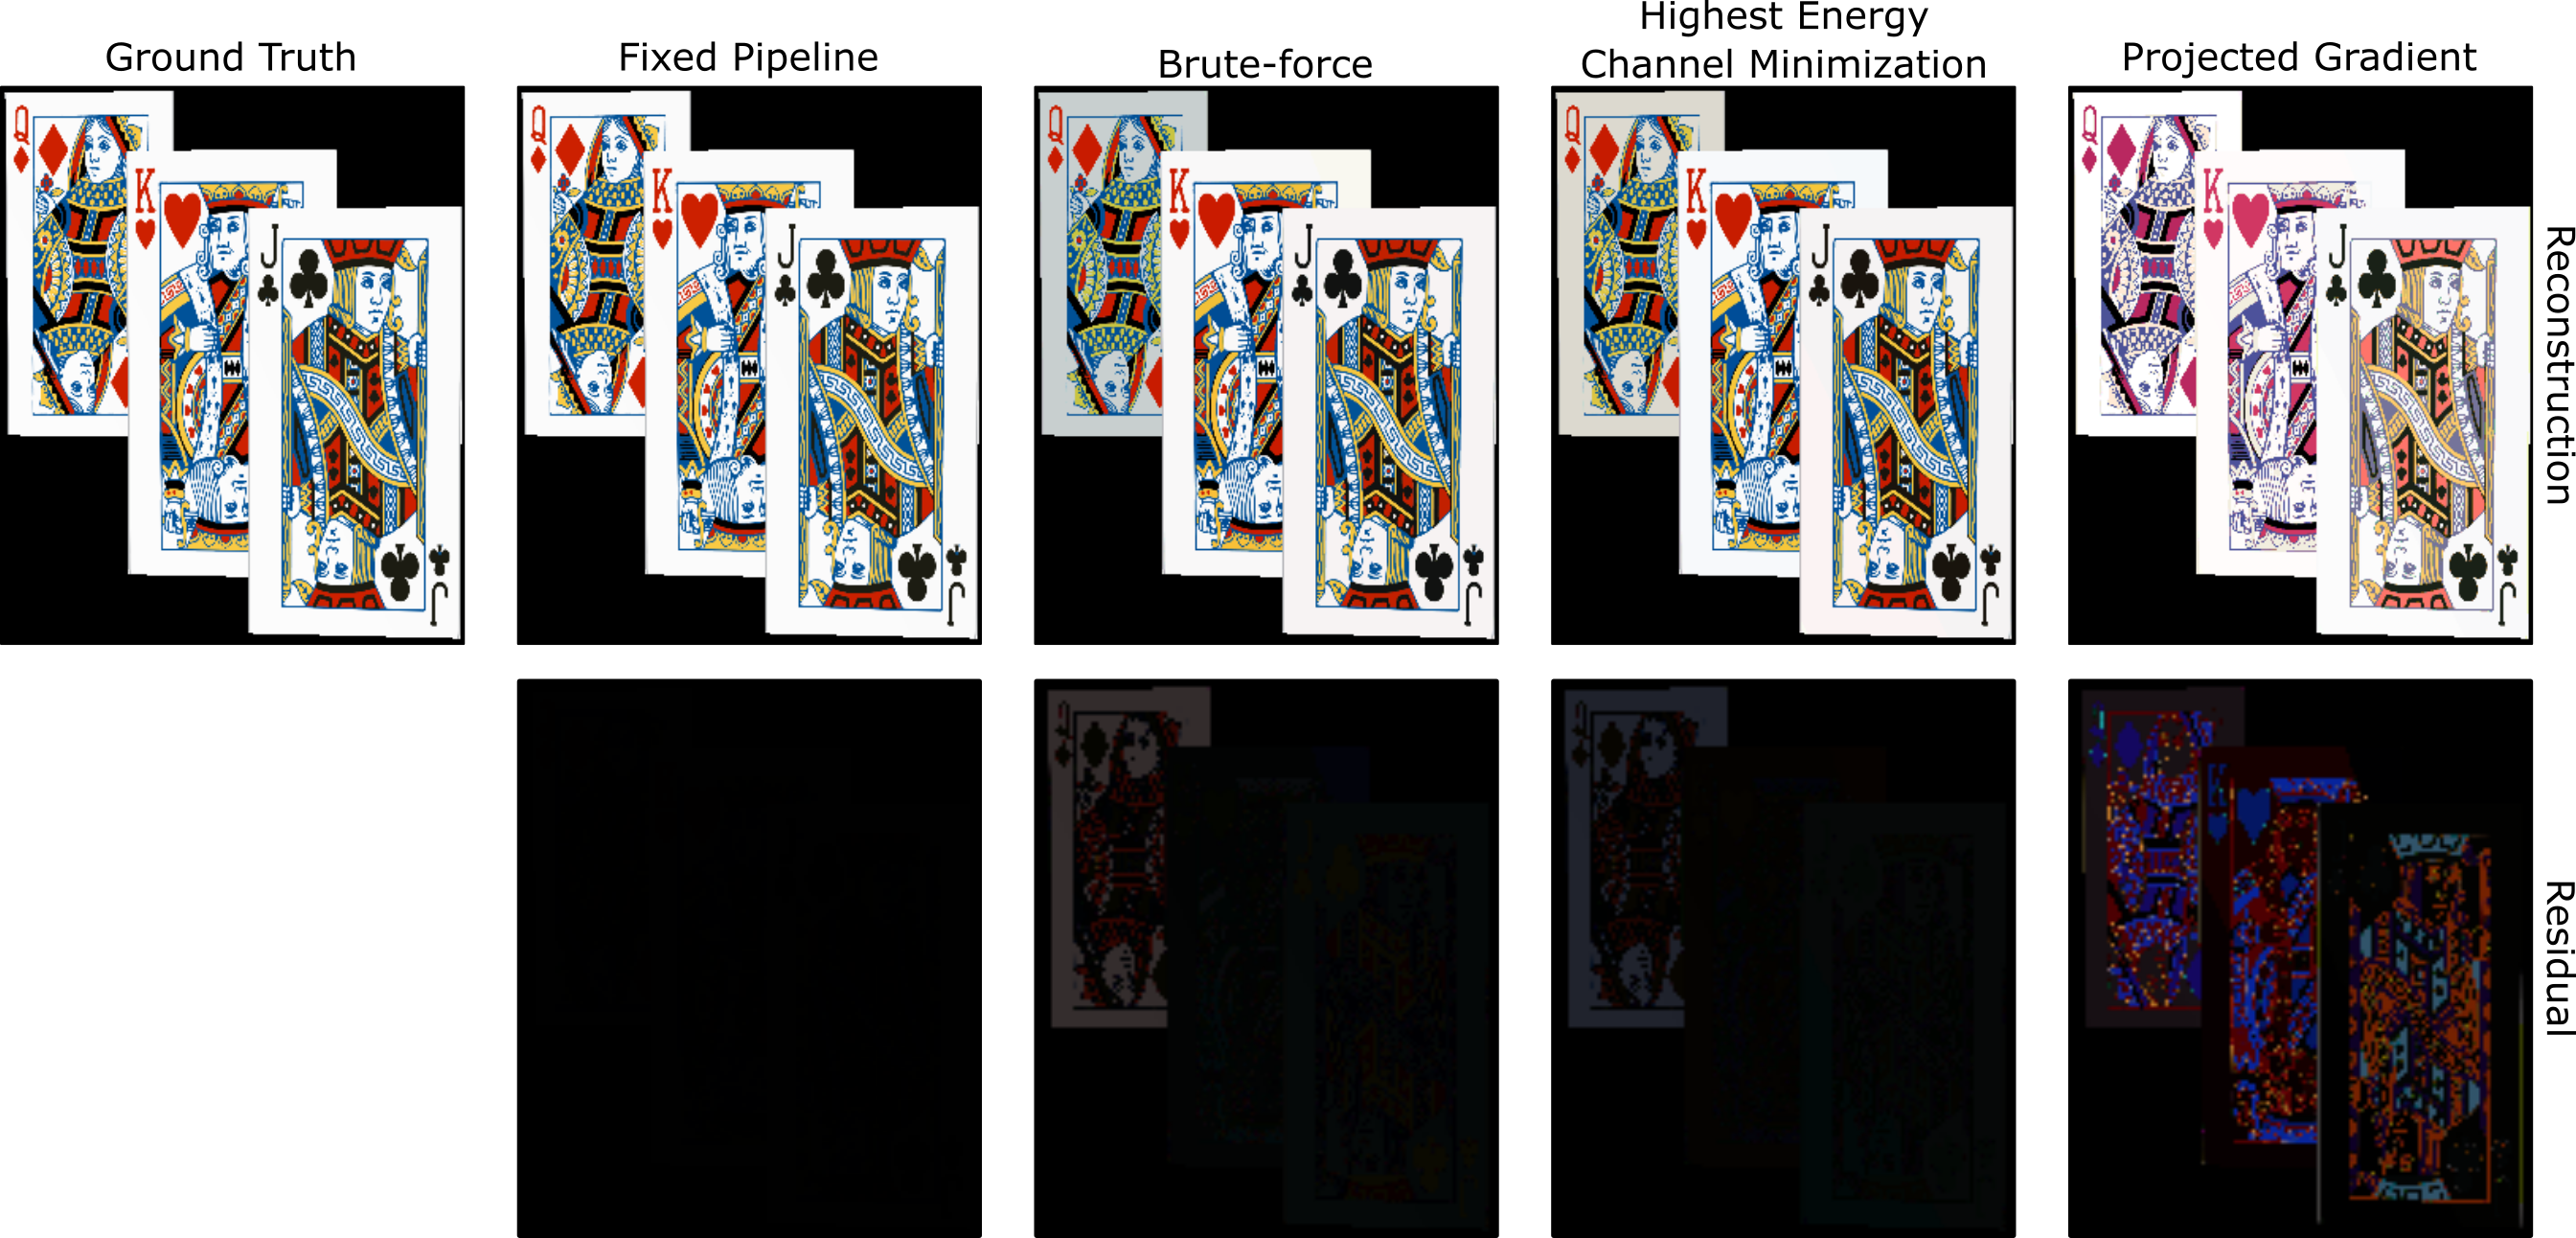
\includegraphics[width=0.99\columnwidth]{images/volumetric/cad_results/cad_visual_quality}
\caption[Color Adaptive Decomposition: visual quality]{Simulation results showing visual quality for the different color adaptive decomposition algorithms.}
\label{fig:volumetric:cad:visual_quality}
\end{figure}


\begin{figure}[h!]
\centering
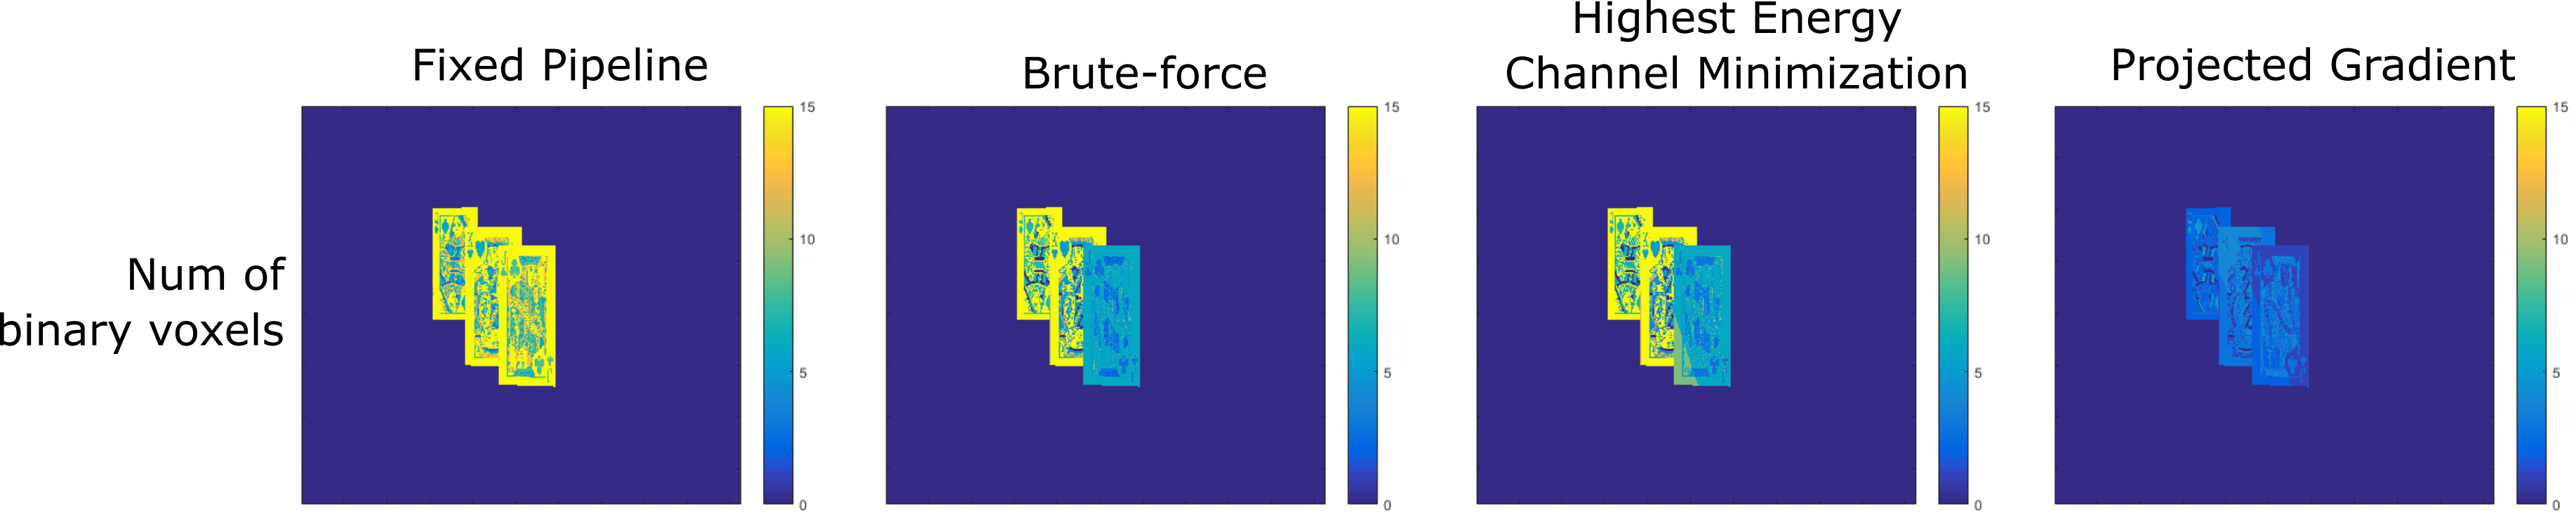
\includegraphics[width=0.99\columnwidth]{images/volumetric/cad_results/cad_num_binary_voxels}
\caption[Color Adaptive Decomposition: number of binary voxels]{Simulation results showing the number of binary voxels needed to represent a color voxel for the different color adaptive decomposition algorithms.}
\label{fig:volumetric:cad:num_binary_voxels}
\end{figure}


Fig.~\todo{rename} compares the number of binary voxels needed to present each color voxel for the different algorithms above. Fig.~\todo{rename} compares the reconstructed image quality and residual images for the different algorithms above. Note that while the \emph{Fixed pipeline} approach gives the best visual quality, the \emph{Projected gradient} approach gives the least number of binary voxels needed to present each color voxel. The \emph{Fixed pipeline} approach gives a residual of zero because it is a deterministic algorithm where the binary volume is guaranteed to fully represent the color volume.

\subsection{Future Work}
\todo{Polish up these things} Above approaches are slow. Opportunity to apply Deep Neural Networks. Global optimization is another direction.
